
%%%%%%%%%%%%%%%%%%%%%%%%%%%%%%%%%%%%%%%%%%%%%%%%%%%%%%%%%%%%%%%%%%%%%%%%%%%%%%%%
%%%%%%%%%%%%%%%%%%%%%%%%%%%%%%%%%%%%%%%%%%%%%%%%%%%%%%%%%%%%%%%%%%%%%%%%%%%%%%%%
\section{Elementos da dança}
\index{Elementos da dança}
\index{Rudolf Laban}
\begin{wrapfigure}{l}{0.30\textwidth}
\vspace{-10pt}
\centering
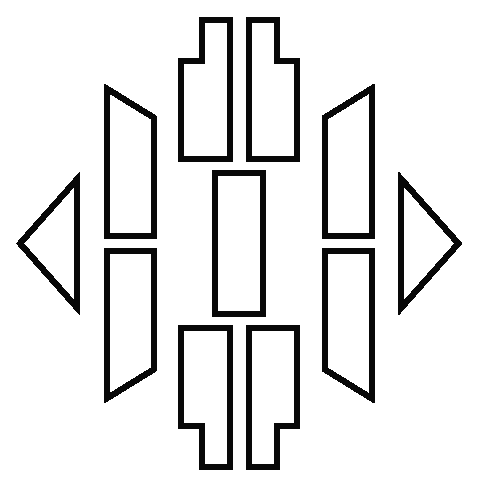
\includegraphics[width=0.28\textwidth]{chapters/cap-dance-elements/Labanotation2.eps}
\caption{Símbolos de Labanotation.}
\label{fig:elementosdanca1old}
\vspace{-10pt}
\end{wrapfigure}
 No seu estudo da teoria do movimento, Rudolf Laban (1879-1958) fez significativas contribuições e
observações na área da ``dança  educacional'',  
realizando contribuições como, a criação de uma forma escrita de notação coreográfica (Labanotation), 
e um  analises preciso do movimento na dança, entre outros \cite[pp. 18]{elementosdanca2017} \cite[pp. 11]{paine2014complete}.

Com seu estudo do movimento, 
Laban  deu sustento ao ensino da dança educativa moderna e 
presentou 16 temas ou áreas-chave no analises do movimento, 
sendo estes ligados a estágios no desenvolvimento das crianças  \cite[pp. 12]{paine2014complete}.

Nas décadas dos anos 1960 e 1970, 
viu-se  na Grã-Bretanha um crescimento importante na dança contemporânea;
a popularidade deste estilo foi devido a que este era menos exclusivo que o balé, 
com técnicas baseadas em movimentos mais naturais, 
além de ter a vantagem de ser unissex e pouco pretensioso.
Assim, estabelecimentos como a ``London School of Contemporary Dance'',
ou bailarinos treinados trabalhando de forma independente,
ofereciam oficinas para faculdades e escolas,
dando um ``enfoque profissional à dança'' \cite[pp. 12]{paine2014complete}.

\begin{wrapfigure}{r}{0.37\textwidth}
\centering
\vspace{-15pt}
%%\smartdiagram[bubble diagram]{Dança, Corpo, Tempo, Espaço, Relações, Dinâmicas}
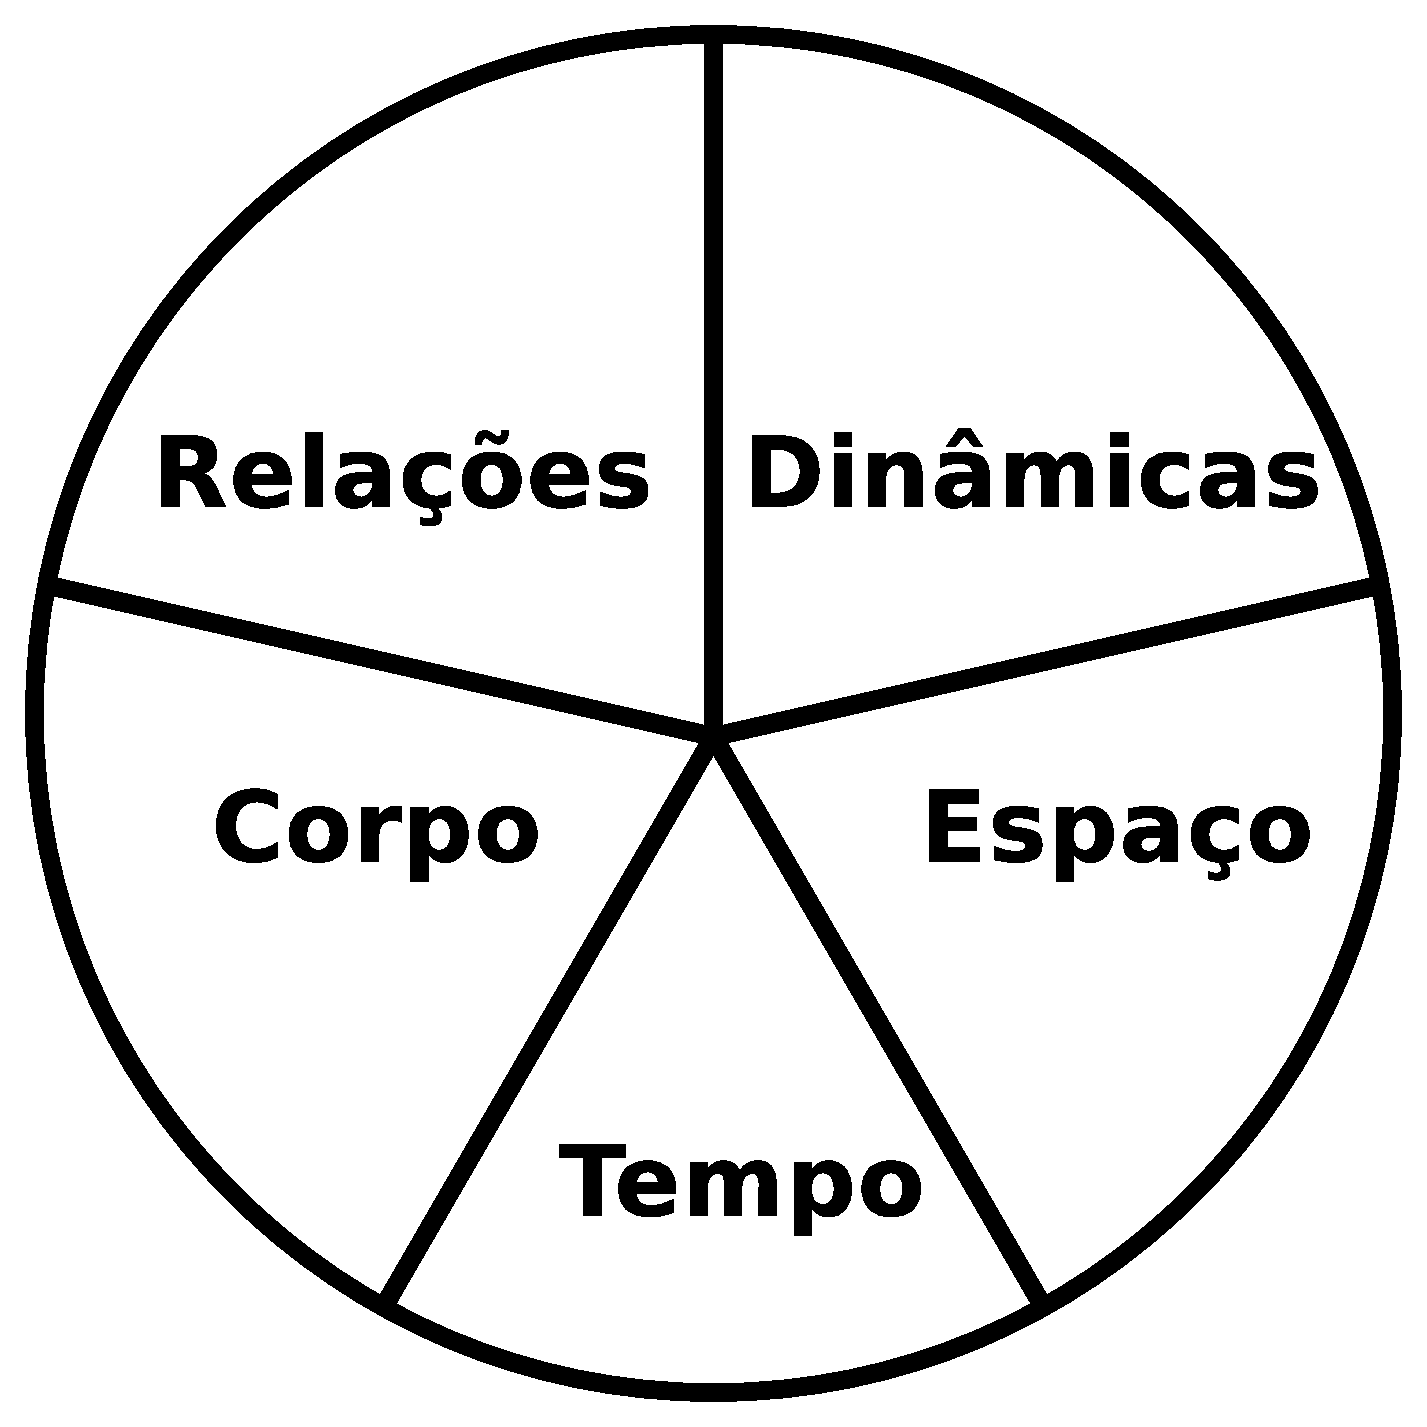
\includegraphics[width=0.35\textwidth]{chapters/cap-dance-elements/DanceElements.eps}
\caption{Elementos da dança}
\label{fig:elementosdanca1}
\vspace{-10pt}
\end{wrapfigure}
Por outro lado, em 1994, Jacqueline Smith-Autard, uma das principais educadoras britânicas de dança, 
propôs um modelo intermediário (``midway model''), entre o educacional e o profissional, 
usando as áreas mais interessantes propostas por Laban \cite[pp. 12]{paine2014complete}.

Seguindo esses modelos, é comum achar na literatura atual 
\cite[pp. 4]{carline2011lesson}       %% corpo, espaço, esforço , relacionamentos
\cite[pp. 13,27]{paine2014complete}   %% corpo, espaço, esforço , relacionamentos
\cite[pp. 69]{schrader2005sense}      %% tempo, espaço, esforço
\cite[pp. 131]{mccutchen2006teaching},%% tempo, corpo, espaço, esforço , relacionamentos
 análises  da dança dividindo esta entre três a cinco elementos,
dependendo da visão do autor.
Estes elementos da dança são: O corpo, as dinâmicas, o espaço, os relacionamentos, e o tempo;
a Figura \ref{fig:elementosdanca1} mostra uma representação gráfica destes elementos.



%%%%%%%%%%%%%%%%%%%%%%%%%%%%%%%%%%%%%%%%%%%%%%%%%%%%%%%%%%%%%%%%%%%%%%%%%%%%%%%%
\subsection{Corpo}
\caracterelement{Do corpo ou das ações}{O que o corpo está fazendo?}
Na dança existem muitos motivos para realizar uma ação corporal;
cada um destes motivos procura ter um significado, seja este prático ou estético, literal ou metafórico \cite[pp. 5]{carline2011lesson}.
As ações realizadas pelo corpo são moldadas pelas relações com os outros elementos da dança,
como as dinâmicas, o uso do espaço, o tempo, e as relações com os outros \cite[pp. 5]{carline2011lesson}.
Algumas das ações mais básicas que podemos realizar com o corpo são,
desloca-nos, pular, virar-nos, gesticular, ou quietude \cite[pp. 27]{paine2014complete}.

\textbf{Deslocamentos:} Implica a transferência do peso do corpo 
para variar de posição no espaço usando na dança;
existem várias formas de realizar esta ação,
por exemplo podemos faze-o pisando, deslizando, rastejando \cite[pp. 28]{paine2014complete}.

\textbf{Pular:} (ou elevar-nos) descreve a ações que provocam que o corpo saia e volta ao chão,
impulsando-nos pelo uso das pernas; as distancias alcançadas podem ser pequenas ou longas,
dependendo do método que usemos no movimento  \cite[pp. 28]{paine2014complete}. 

\textbf{Virar:} envolve movimentos de rotação em torno de um eixo.
Este giro não tem que ser necessariamente completo ($360^o$),
e podem ser trabalhados níveis, como giros de um ângulo especifico;
os movimentos de giro podem ser iniciados por alguma parte do corpo, 
não necessariamente pelos pés \cite[pp. 29]{paine2014complete}.

\textbf{Gesto:} Implica o movimento de uma ou varias partes do corpo,
que não envolve suporte ou transferência de peso
(ex: movimentos axiais, como flexão, alongamento e torção);
os gestos enriquecem o conteúdo expressivo de uma dança,
onde são usados para contar uma história, 
usando um vocabulário simbólico reconhecido popular ou tradicionalmente 
\cite[pp. 29]{paine2014complete}.

\textbf{Quietude:} descreve a capacidade de interromper nosso movimento, 
controlando no processo nosso equilíbrio \cite[pp. 29]{paine2014complete}.


A consciência corporal se centra no estudo do uso controlado do corpo, 
à medida que as movimentações são exploradas,
já sejam  estes movimentos realizados pelo corpo inteiro,
ou por partes isoladas deste \cite[pp. 5]{carline2011lesson}.
O tema da consciência corporal será abordado com maior aplitude  na Seção \ref{sec:BodyAwareness}.


%%%%%%%%%%%%%%%%%%%%%%%%%%%%%%%%%%%%%%%%%%%%%%%%%%%%%%%%%%%%%%%%%%%%%%%%%%%%%%%%
\subsection{Dinâmica (esforço)}
\caracterelement{Das dinâmicas}{Como o corpo está se movendo?}
As dinâmicas no movimento 
indicam o jeito em que a energia será usada e direcionada no corpo durante a dança \cite[pp. 131, 136]{mccutchen2006teaching};
além de provocar em nossos movimentos algo que poderia ser definido, metaforicamente, como textura ou cor;
dando uma identidade própria a cada movimento, dependendo da dinâmica utilizada;
por exemplo, não é o mesmo dar um passo de forma lenta como tentando não fazer barulho,
que dar o passo caindo como se estivéssemos bêbados.

Rudolf Laban, no seu estudo do movimento, 
dividiu as dinâmicas (ou ``esforço'' na notação de Laban) 
em quatro categorias ou fatores: peso, tempo, espaço e fluxo 
\cite[pp. 5]{carline2011lesson}
\cite[pp. 30]{paine2014complete}.
Porém, o modelo de Laban não é a única forma em que podemos fatorar as dinâmicas,
de modo que, inclusive a escolha do modelo para descrever as dinâmicas,
influencia na textura percebida na realização do movimento \cite[pp. 30]{paine2014complete}. 

Uma explicação detalhada, dos fatores nos quais podemos dividir as 
\hyperref[subsec:fatordinamica]{\textbf{dinâmicas do movimento}},
pode ser encontrada na Seção \ref{subsec:fatordinamica};
com este propósito serão mostrados diferentes modelos propostos por vários autores,
sobre como podem ser fatoradas as dinâmicas.



%%%%%%%%%%%%%%%%%%%%%%%%%%%%%%%%%%%%%%%%%%%%%%%%%%%%%%%%%%%%%%%%%%%%%%%%%%%%%%%%
\subsection{Espaço} 
\caracterelement{Do espaço}{Para onde o corpo se está movendo?}
A maneira como o espaço é usado pode ajudar a dar interesse visual a nossa dança,
ajudando-nos a contar uma historia como nosso corpo, com um relato que progride no tempo 
\cite[pp. 6]{carline2011lesson}
\cite[pp. 31]{paine2014complete}
\cite[pp. 131, 136]{mccutchen2006teaching}; 
alguns aspectos do espaço que podem ser interessantes de ser explorados na nossa dança são:

\textbf{Espaço pessoal e geral:}  Trabalhamos no nosso espaço pessoal 
quando realizamos movimentos sem deslocamento 
(ex: tremer, subir, girar, pausar ou afundar);
e em nosso espaço geral quando nos deslocamos a outras posições
(ex: caminhar, correr, pular) \cite[pp. 7]{carline2011lesson}
\cite[pp. 32]{paine2014complete}.

\textbf{Caminhos:} Podemos definir o caminho como o padrão desenhado no chão ou no ar, 
quando nos deslocamos,
esta padrão pode ser uma única linha reta ou 
varias conectadas formando padrões mais complexos, 
 com zigue-zagues; também poderíamos ter caminhos curvos e sinuosos; 
inclusive o caminho pode ser uma curva sem inicio né fim como um círculo 
\cite[pp. 7]{carline2011lesson}
\cite[pp. 32]{paine2014complete}.



\textbf{Direções:} Quando trabalhamos com direções, 
temos a possibilidade que nosso movimento seja 
para frente, para trás, para os lados, para cima, para baixo, em diagonal,
entre outras 
\cite[pp. 7]{carline2011lesson}
\cite[pp. 32]{paine2014complete}
\cite[pp. 97-98]{schrader2005sense}. 


\textbf{Formas do corpo:} Com nosso corpo, ou grupo de corpos, podemos criar formas diferentes,
como emular uma parede, uma esfera, 
ou podemos fazer posturas mediante torções, 
e movimentando de forma independente distintas partes do corpo 
\cite[pp. 8]{carline2011lesson}
\cite[pp. 32]{paine2014complete}
\cite[pp. 97]{schrader2005sense}.

\textbf{Níveis:} Quando usamos nosso corpo, 
podemos quantificar nossos movimentos em vários níveis,
relacionados com a distancia com o chão;
por exemplo ao pular, este movimento pode ser baixo, meio ou alto 
\cite[pp. 8]{carline2011lesson}
\cite[pp. 32]{paine2014complete}
\cite[pp. 96]{schrader2005sense}.

\textbf{Posição e proximidade:}  (Preposições espaciais)
É possível usar preposições que nos ajudem a descrever, o uso do espaço,
em relação à posição e proximidade; entre os termos que podemos usar temos:
atrás, na frente, 
acima, abaixo, 
perto, longe, 
através, ao redor
\cite[pp. 32]{paine2014complete} 
\cite[pp. 9]{carline2011lesson}, etc.

\textbf{Dimensão} (Tamanho do movimento ou forma) 
Indica a dimensão de grandeza ou amplitude que terá o movimento ou a forma que executemos;
assim, podemos escolher valores de dimensão entre pequeno e grande 
\cite[pp. 32]{paine2014complete} 
\cite[pp. 99]{schrader2005sense}.

%\textbf{Bases do corpo:}  \cite[pp. 8]{carline2011lesson}.

%\textbf{Extensões para o espaço:}  \cite[pp. 9]{carline2011lesson}.

%%%%%%%%%%%%%%%%%%%%%%%%%%%%%%%%%%%%%%%%%%%%%%%%%%%%%%%%%%%%%%%%%%%%%%%%%%%%%%%%
\subsection{Relacionamento} 
\caracterelement{Das relações}{Com quem ou com que o corpo está se movendo?}
Na dança podemos nos movimentar relacionando-nos com outra pessoa, como na dança social a  dois,
ou em grupos, como em algumas danças folclóricas.
Quando dançamos podemos liderar a dança ou ser seguidores, 
também podemos nos deslocar indo ao encontro com o grupo, 
ou nos separar, dividir, espelhar, contrastar, 
estar em cânone, em uníssono, ou alguma outra forma;
a forma de nos relacionar com os demais são variadas,
inclusive podemos interagir como objetos, sejam estes reais ou imaginários
 \cite[pp. 9]{carline2011lesson}
 \cite[pp. 27, 32-33]{paine2014complete}
\cite[pp. 131, 132, 134]{mccutchen2006teaching}.


%%%%%%%%%%%%%%%%%%%%%%%%%%%%%%%%%%%%%%%%%%%%%%%%%%%%%%%%%%%%%%%%%%%%%%%%%%%%%%%%
\subsection{Tempo}
\caracterelement{Do tempo nas ações}{Quando o corpo realiza uma ação?}
O movimento e as pausas que realizamos estão sempre ligados à variável tempo,
tendo estes um tempo inicial e uma duração;
assim, nossos movimentos, vistos de forma sequencial no tempo, 
seguem um ritmo que pode ser marcado livremente por nós,
ou pode tentar seguir uma fonte externa de informação, como a música;
em qualquer caso o dançarino é o encarregado desta escolha criativa;
existem alguns termos que devem ser parte de nosso vocabulário de dança,
quando estudamos o aproveitamento do elemento tempo,
estes são: 
\hyperref[ref:Pulso]{\textbf{pulso}}, 
\hyperref[sec:Tempo]{\textbf{tempo}}, 
\hyperref[sec:Andamento]{\textbf{andamento}}, 
\hyperref[sec:pos:Ritmo]{\textbf{ritmo}}, e 
\hyperref[def:Metrica]{\textbf{métrica}}
\cite[pp. 82]{schrader2005sense}
\cite[pp. 131, 134, 136]{mccutchen2006teaching}.

%%%%%%%%%%%%%%%%%%%%%%%%%%%%%%%%%%%%%%%%%%%%%%%%%%%%%%%%%%%%%%%%%%%%%%%%%%%%%%%
% FALTA INCLUIR ENERGIA
%%%%%%%%%%%%%%%%%%%%%%%%%%%%%%%%%%%%%%%%%%%%%%%%%%%%%%%%%%%%%%%%%%%%%%%%%%%%%%%
%% https://books.google.com.br/books?id=C0yjXGJ3EEoC&pg=PA131&dq=dynamics+dance+energy&hl=pt-BR&sa=X&ved=0ahUKEwjc472wjrXlAhUeEbkGHbstBbUQ6AEIKTAA#v=onepage&q=dynamics%20%20energy&f=false
%% https://books.google.com.br/books?id=omYS0_FkOWIC&pg=PT169&dq=dynamics+dance+energy&hl=pt-BR&sa=X&ved=0ahUKEwjc472wjrXlAhUeEbkGHbstBbUQ6AEIMjAB#v=onepage&q=dynamics%20energy&f=false
%% https://books.google.com.br/books?id=Z0hoAwAAQBAJ&printsec=frontcover&dq=discovering+dance&hl=pt-BR&sa=X&ved=0ahUKEwif04WJwbXlAhUkILkGHdxnAjEQ6AEIKTAA#v=onepage&q=discovering%20dance&f=false
%%%%%%%%%%%%%%%%%%%%%%%%%%%%%%%%%%%%%%%%%%%%%%%%%%%%%%%%%%%%%%%%%%%%%%%%%%%%%%%
%%%%%%%%%%%%%%%%%%%%%%%%%%%%%%%%%%%%%%%%%%%%%%%%%%%%%%%%%%%%%%%%%%%%%%%%%%%%%%%
